\documentclass[12pt]{article}
\usepackage{graphicx} % Required for inserting images
\graphicspath{{../results}}
\usepackage{csvsimple}
\usepackage{booktabs}
\usepackage{subcaption}
\usepackage{setspace}
\usepackage{lineno}
\usepackage{amsmath}
\usepackage{verbatim}
\usepackage{textcomp}
\usepackage{float}

\nonstopmode
\newcommand\wordcount{\input{WordCount.sum}}

\title{\vspace{-2cm}Temperature Does Not Affect Model Performance when Predicting Microbial Population Growth}

\author{Sam Smith}

\date{}
\onehalfspacing

\begin{document}
\begin{titlepage}
  
  \maketitle
  
  \begin{center}
    Department of Life Sciences \\ Imperial College London \\ SW7 2AZ \\ UK
    \end{center}

    \begin{center}
      Word Count: \wordcount
    \end{center}

  \begin{abstract}
    Microorganisms constitue the most diverse and abundant life forms on Earth. Interest in their role on maintaining ecosystem function has grown in the context of climate change. This report aims to identify the best performing microbial population growth model between Gompertz, Logistic and cubic models. Moreover, trends between model performance and temperature will be inspected. 285 microbial population curves, grown under a range of environmental conditions were fit to the three models and model selection analyses were carried out. It was found that the Gompertz model was overall the strongest performer with no clear observable trends with temperature for any model. Though Gompertz was the best performer overall, the absence of a clear winner, suggested microbial populations are best predicted by models with parameters that align with the features of a specific curve. Thus explaining the use of many different models in the literature.
  \end{abstract}
\end{titlepage}

  \section{Introduction}
  \linenumbers
Microorganisms make up the most diverse and plentiful group of life on Earth. They are essential for ecosystem function and stability \cite{Shoemaker2021}. In particular microbes play a critical role in processes such as the nitrogen cylcle and carbon sequestration that are becoming increasingly significant in light of climate change \cite{Gupta2016}. Microbes have immense ability to multiply rapidly and exponentially whilst resources are abundant. As nutrients become limited, microorganisms must compete thus compromising their ability to reproduce \cite{NatRevMicro}. This results in them typically showing a sigmoidal pattern of growth whereby different stages of their growth curve infer different biology significance. Microbial growth curves typically consist of a lag phase (tlag), exponential growth phase, stationary phase (K), and often a death phase \cite{Zwietering1990}. The lag phase accounts for the time taken for a population to adjust to its environment before rapid reproduction \cite{BUCHANAN1997313}. Whereas, the stationary phase or carrying capacity is shown as an asymptote on a bacterial growth curve and indicates often compounding factors such as nutrient availability, predation, and crowding preventing further population growth \cite{WACHENHEIM2003157}. The maximum growth rate (Rmax) is also typically annotated on microbial growth curves, illustrated by the steepest gradient.\\
     
Models can be developed that effectively predict microbial populations at a given time point. They work under the assumption that microbial population patterns are reproducible under the same environmental conditions \cite{Pla2015}. Modelling microbial population dynamics has positive implications on agriculture and food security, as predictions on shelf life and product safety can be made \cite{Zwietering1990}. In addition, predictive models assist in the decision making of large industrial processess such as fermentation \cite{Garcia2021}. Models that are derived from existing theory and recorded observations are known as mechanistic; whilst phenomenological models are developed empirically and provide no explanation of patterns \cite{doi:10.1080/10408398.2011.570463}. Two examples of commonly used non-linear mechanistic models are the the Gompertz model and the Logistic model.\\

The Logistic equation is popular for describing bacterial population growth. The Logistic model that was first developed by Pearl and Reed in 1920 was emperical. However, biological inferences are now commonly derived from its parameters \cite{WACHENHEIM2003157} \cite{Pearl1920}. Therefore, it can be said that the Logistic model estimates the population at any given time point from the initial population ($\mathrm{N}_0$), K and Rmax values \cite{WACHENHEIM2003157}. Whilst models consisting of fewer parameters are often preferred, the Logistic equation does lack parameters that captivate other typical stages of microbial growth curves such as a death or lag phase. The Gompertz equation is another sigmoidal model that takes into account the three parameters in the Logistic model but also includes a tlag. The Gompertz model has been widely used across a range of applications such as predicting plant, fish or even cancerous tumour growth \cite{Tjrve2017}. Finally, phenomenological cubic linear models are often used for predicting microbial populations. Garcia et al (2021) found that a cubic model accurately represents all aforementioned stages of bacterial population growth when applied to fermentation bacteria \cite{Garcia2021}. However, biological inferences cannot be drawn from phenomoligcal model parameters, highlighting the importance of mechanistic models that provide parameter estimations, as well as predictions.\\

Statistical analysis whereby different models are selected or ranked in terms of performance have begun to gain traction in ecology and evolution \cite{JOHNSON2004101}. It offers an alternative to traditional hypothesis testing techniques as it confronts multiple `competing' hypotheses simultaneously. It is crucial to identify the best performing models under various conditions, as the prediction of microbial population dynamics relies on selecting the best performing model that aligns with the conditions of unsampled populations. This report aims to identify trends in model performance between cubic, Gompertz and Logistic, under different temperatures. It is expected that the Gompertz model may drop in performance relative to the Logistic model with increasing temperatures. This is due to the tlag being significantly reduced by increasing temperatures \cite{ABA2021109108} as populations can adapt to new conditions faster. Furthermore, I expect no changes in model perfomance for the Cubic model across temperatures as its parameters are not tied to any biological variables that are temperature dependent. Temperature is also known to influence the Rmax \cite{Ward1972} \cite{Dey2020}. Rates of substrate uptake by bacteria reduce with lower temperatures thus negatively impacting a bacteria's ability to grow \cite{Nedwell1994}. However as both mechanistic models contain an Rmax parameter this should not vary relative model performance.\\

Finally, the model averaging application of model selection techniques will be carried out in this study. Robust parameter estimates for K and Rmax will be calculated using Akaike weights for demonstration and use in potential follow up studies.

\section{Methods}

    \subsection{Data Collection}
This study is based on an amalgumation of microbial growth curves from 10 different research papers. It includes populations of different species grown under varying temperatures (0 - 37C) and 18 different media. Observations in the dataset were deemed from the same curve if they shared a temperature, species and citation. This facilitated the subsetting of the data into 285 individual growth curves for model fitting.

    \subsection*{Model Fitting}
Only three canditate models were considered in this study as it is ill-advised to include many models that increase the chance of spurious findings \cite{JOHNSON2004101}. The Logistic model used in this study is the solution to the differential equation defining the classic Logistic population growth equation.
    \subsubsection{Logistic Model}
    \begin{equation}
        N_t = \frac{N_0Ke^{r_{max}t}}{K+N_0(e^{r_{max}t} - 1)}
      \end{equation}
The Gompertz model used in this study is a modified version by Zwietering et al (1990) \cite{Zwietering1990} where Nmax represents carrying capacity. 
    \subsubsection{Gompertz Model}
    \begin{equation}
        log(N_t) = N_0 + (N_{max}-N_0)e^{-e^{r_{max}exp(1)\frac{t_{lag}-t}{(N_{max}-N_0)log(10)}+1}}
        \end{equation}
Finally, the equation below illustrates the cubic equation and its uninterpretable parameters.
    \subsubsection{Cubic Model}
    \begin{equation}
        log(N_t) = at + bt^2 + ct^3 + d
    \end{equation}

Fitting the non linear mechanistic models (Logistic and Gompertz) required reasonable starting values in addition to suitable upper and lower bounds. Sampling was used to vary the starting values around an appropriate mean to increase the likelihood of a non-linear least squares (NLLS) model fit after 100 attempts. After the 100 attempts for each growth curve, only the fit with the highest $\mathrm{R}^2$ value was outputted alongside its respective AICc, BIC, and Akaike weight ($\mathrm{A}_{\textit{W}}$) score. All three models were managed to be fit to 202 out of 285 growth curves. For consistency, when working out the statistical metrics for the Logistic model, the residuals were log transformed to facilitate comparison between the other models. In addition, log transformed population data is prefered as population is a multiplicative process therefore residuals naturally increase with time in a linear scale. This will increase the uniformality of the model residuals which leads to consistent predictive power across the range of time values \cite{Freckleton2002}.


    \subsection{Model Comparison and Weighted Averages}
Johnson and Omland outlined model selection metrics and described the differences between them. Firstly, $\mathrm{R}^2$ is used that simply suggests the proportion of the variance in the data that is explained by a given model. $\mathrm{R}^2$ is not commonly used and is described as `naive' as it does not consider model complexity and therefore does not penalise overfitted models \cite{JOHNSON2004101}. Secondly, Akaike information criterion (AIC) is another measure of model performance that counts for goodness of fit and model complexity. Furthermore, AICc includes bias correction when the model is applied to small sample sizes. Finally bayesian information criterion (BIC), similar to AICc, considers fit, complexity and sample size. However, AIC is often favoured as it is based on Kullback-Leibler information theory \cite{JOHNSON2004101} - though some statisticians still argue that BIC is preferable as it is less tolerant of overcomplex models. When comparing model AIC and BIC values, models with the smallest AIC and BIC by at least 2, are considered the better performing model \cite{JOHNSON2004101}. Model comparison occurs between models fit onto the same data and an overall model winner is defined as the model that performed best the most number of times. In addition, model performances were compared under all different temperature values to identify trends in model performance.\\

Omland and Johnson further explain the use of a more interpretable metric, Akaike weights that consider the relative probabilities of a model being the best performer. In this study, for a model to be selected as the best performer an $\mathrm{A}_{\textit{W}}$ score of over 0.9 is necessary \cite{DASH2023103140}. This is an arbitrary threshold suggesting a model can only be deemed the best if there is more than 90 percent chance that that is the case. These probabilities can consequently be used for robust parameter estimations. In this study, $\mathrm{A}_{\textit{W}}$ averages were made for comparison between all three models. However, for parameter estimations $\mathrm{A}_{\textit{W}}$ were recalculated for just Gompertz and Logistic as the Cubic model does not contain interpretable parameters associated with stages of bacterial growth.

\subsection{Computational Tools}

Firstly the pandas package in python 3.10.12 \cite{10.5555/1593511} was used for initial data manipulation and exportation as it is a computationally efficient and popular tool. R version 4.1.2 \cite{R} was consequently used for model fitting,  analysis, and plotting. For NLLS model fitting, minpack.lm package was used to access the nlsLM function that uses the Levenberg-Marqualdt algorithm, known to be more robust than the Gauss-Newton algorithm. The purrr package, which incorporates the possibly function, was employed to continue the iterative process in the model fitting and plotting functions in the presence of errors. The dplyr package was used for appending model winners to respective IDs before tables and graphs could be plotted. Finally, ggplot2 was used for producing all graphs included in the report.

\section{Results}
All 202 growth curves with fitted models were plotted with both log transformed and linear population values. Subset 225 is a good example for illustrating the differences between plot types:

\begin{figure}[H]
    \centering
    \begin{subfigure}{0.5\textwidth}
      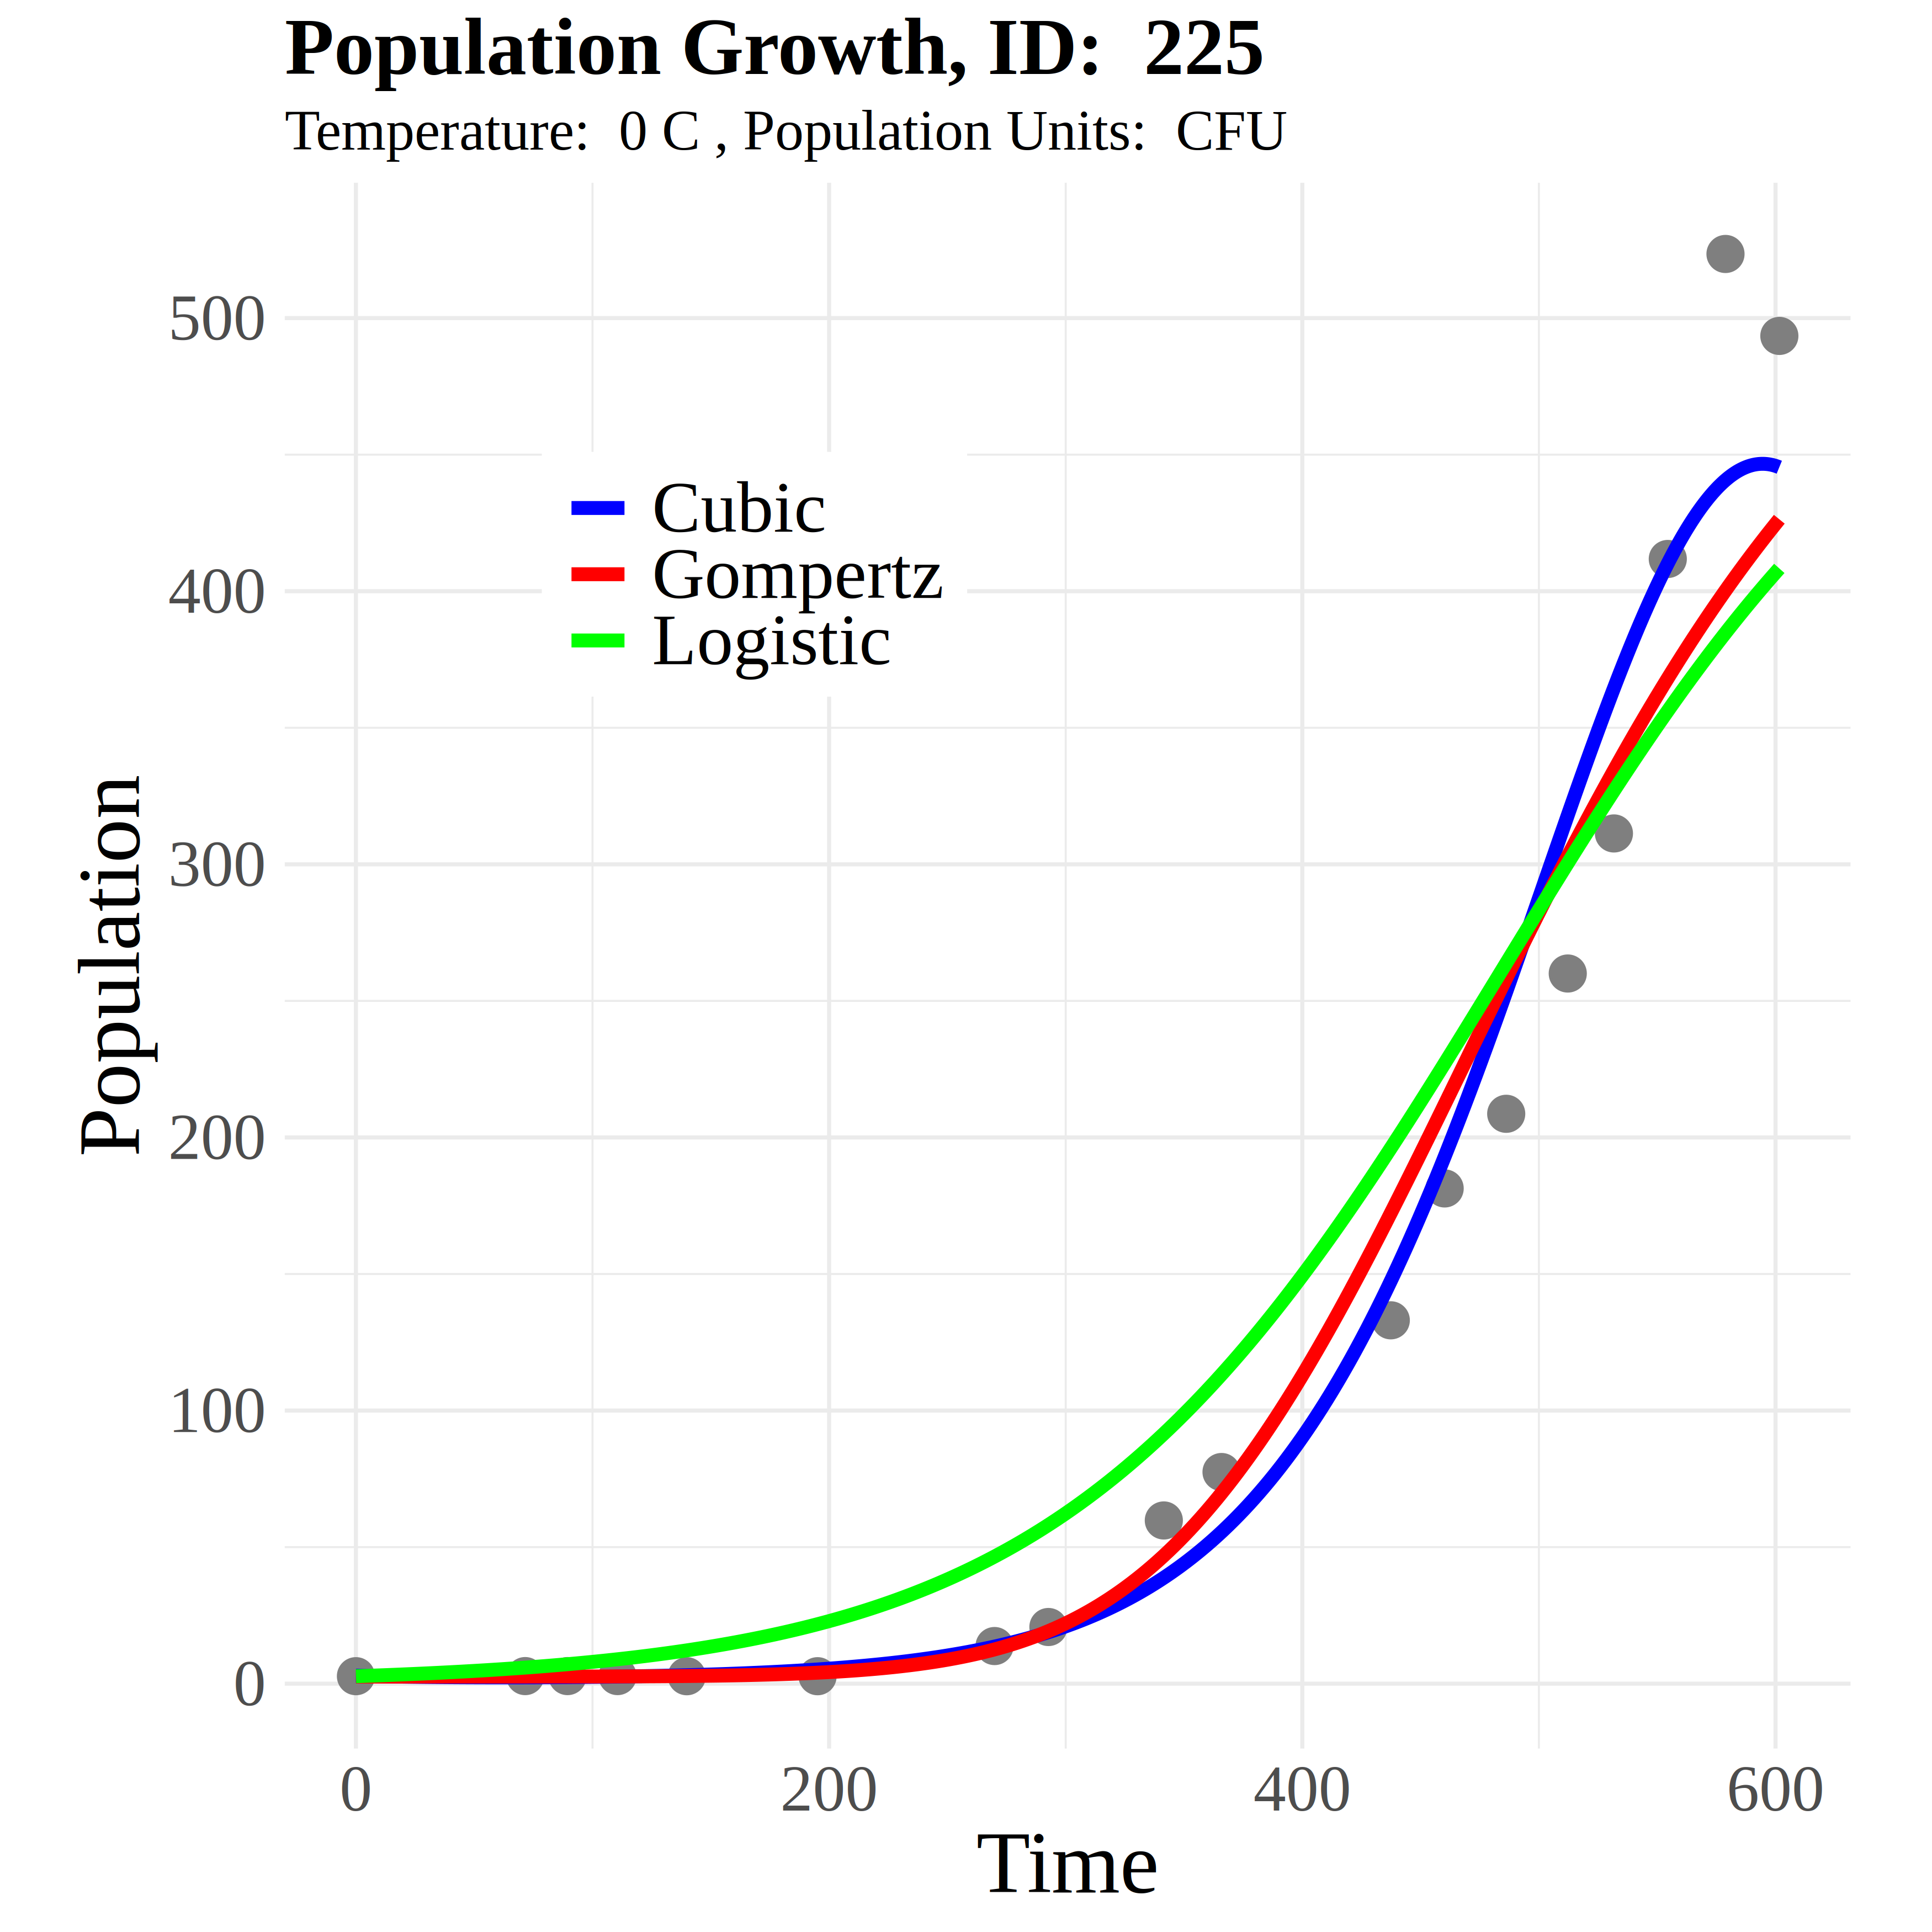
\includegraphics[width=\linewidth]{LinearMod.png}
      \caption{Population against Time}
    \end{subfigure}%
    \begin{subfigure}{0.5\textwidth}
      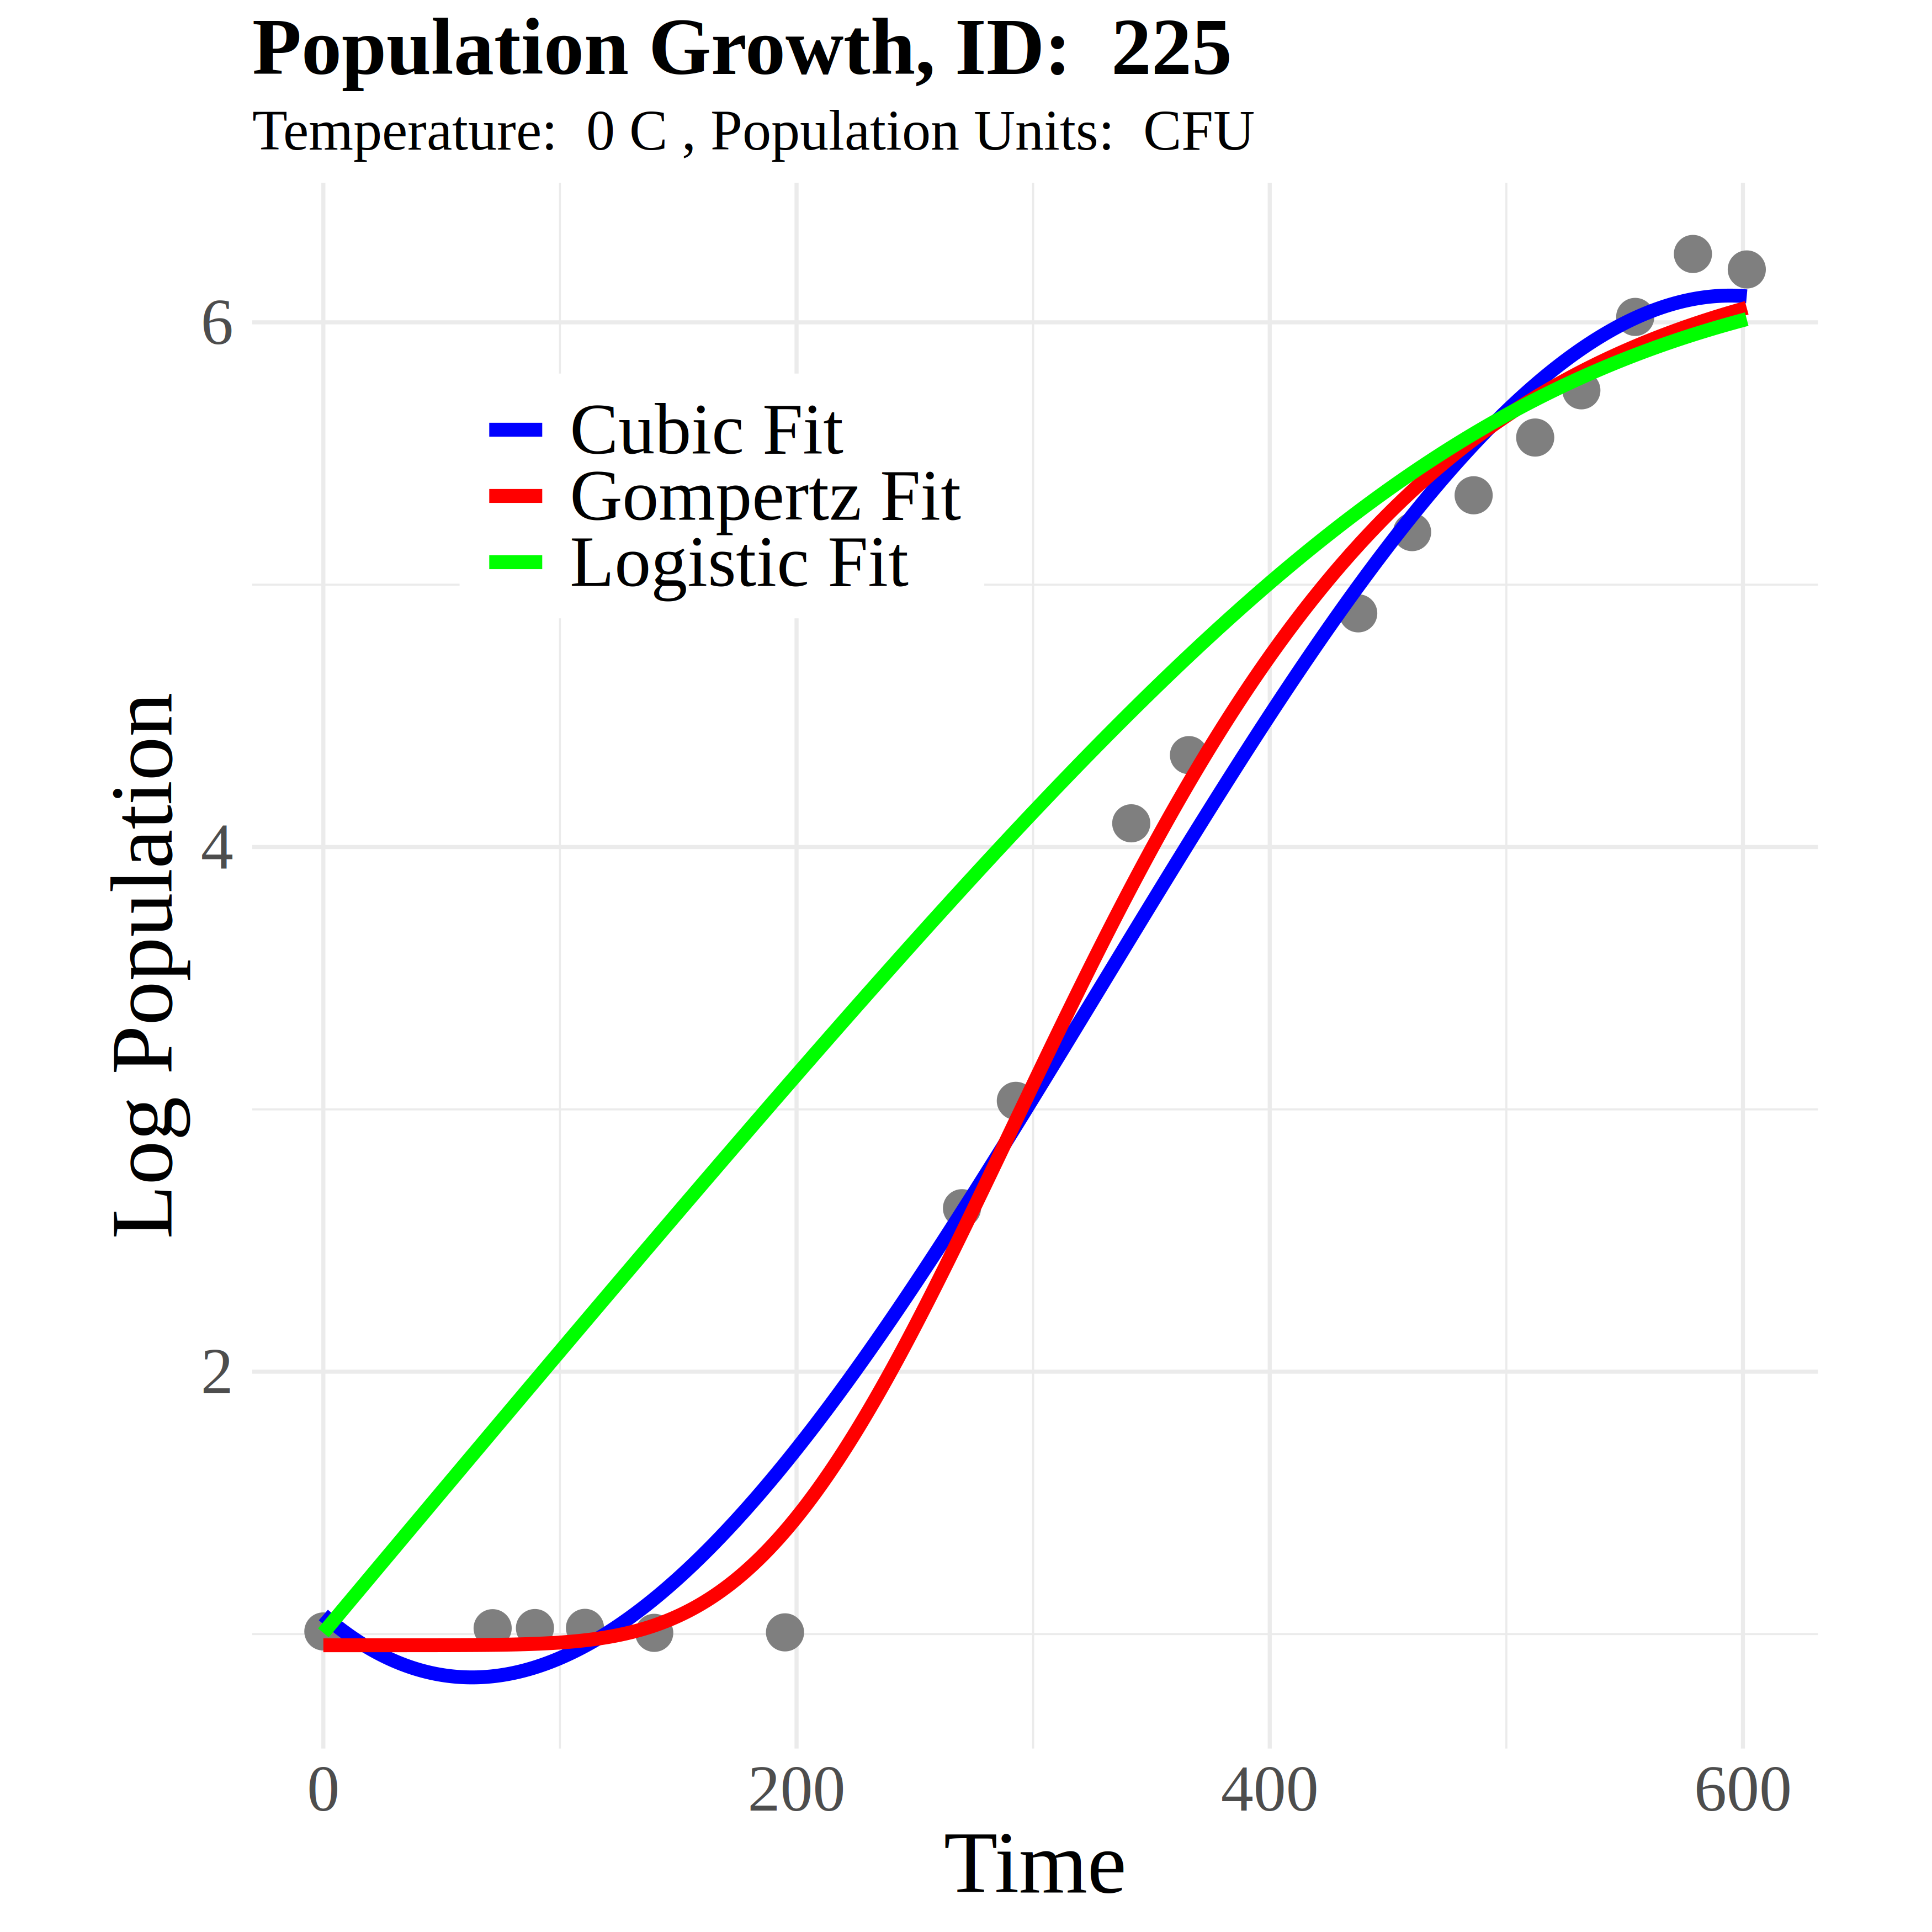
\includegraphics[width=\linewidth]{LogMod.png}
      \caption{Log Population against Time}
    \end{subfigure}
    \caption{Graphs showing the relationship between log and linear microbial populations against time for subset 225.}
\end{figure}

In both plots it is clear that the Gompertz and Cubic models were best fit to the data. This would suggest their $\mathrm{R}^2$ values would be stronger however, as the Logistic model contains fewer parameters, AIC and BIC values may tell a different story. Furthermore, both plots illustrate the Logistic models struggle to fit curves with a time lag phase. The Gompertz and Cubic manage to captivate the lag phase, growth phase and stationary phase, with the cubic even predicting a death phase shown by a slight decline in predicted population.\\

The number of times each model performed best for a given criteria is shown in this table below: 

\begin{table}[H]
  \centering
  \csvreader[
    head to column names,
    tabular=|c|c|c|c|c|,
    table head=\toprule \textbf{Model} & \textbf{AICc} & \textbf{BIC} & $\mathrm{R}^2$ & $\mathrm{A}_{\textit{W}}$ \\ \midrule,
    table foot=\bottomrule,
    late after last line=\\\bottomrule]
  {../results/bestmodeltable.csv}
  {1=\Model, 2=\AICc, 3=\BIC, 4=\Rsqrd, 5=\Aw}
  {\Model & \AICc & \BIC & \Rsqrd & \Aw}
  \caption{The number of top performances for all models according to each criteria}
\end{table}

Table 1 shows that Gompertz was the best performing model the most number of times for each criteria. The Gompertz model's quality of fit clearly outweighed its penalty for having an extra parameter than the Logistic model for AICc and BIC. Furthermore, the Cubic and Gompertz models clearly outperformed the Logistic according to $\mathrm{R}^2$ , aligning with expectations due to their greater number of parameters. Despite this, the number of $\mathrm{A}_{\textit{W}}$ best fits is fairly similar across all three models. The Gompertz model had a probability of being the best model of more than 0.9 only 59 times out of the 202 growth curves. It is important to note that the columns may not add up to 202 due to 'no clear winner' outcomes where threshold values were not attained.\\

The propotions of best fits for each model were calculated and plotted for each unique temperature value in the dataset. 
\begin{figure}[h]
  \centering
  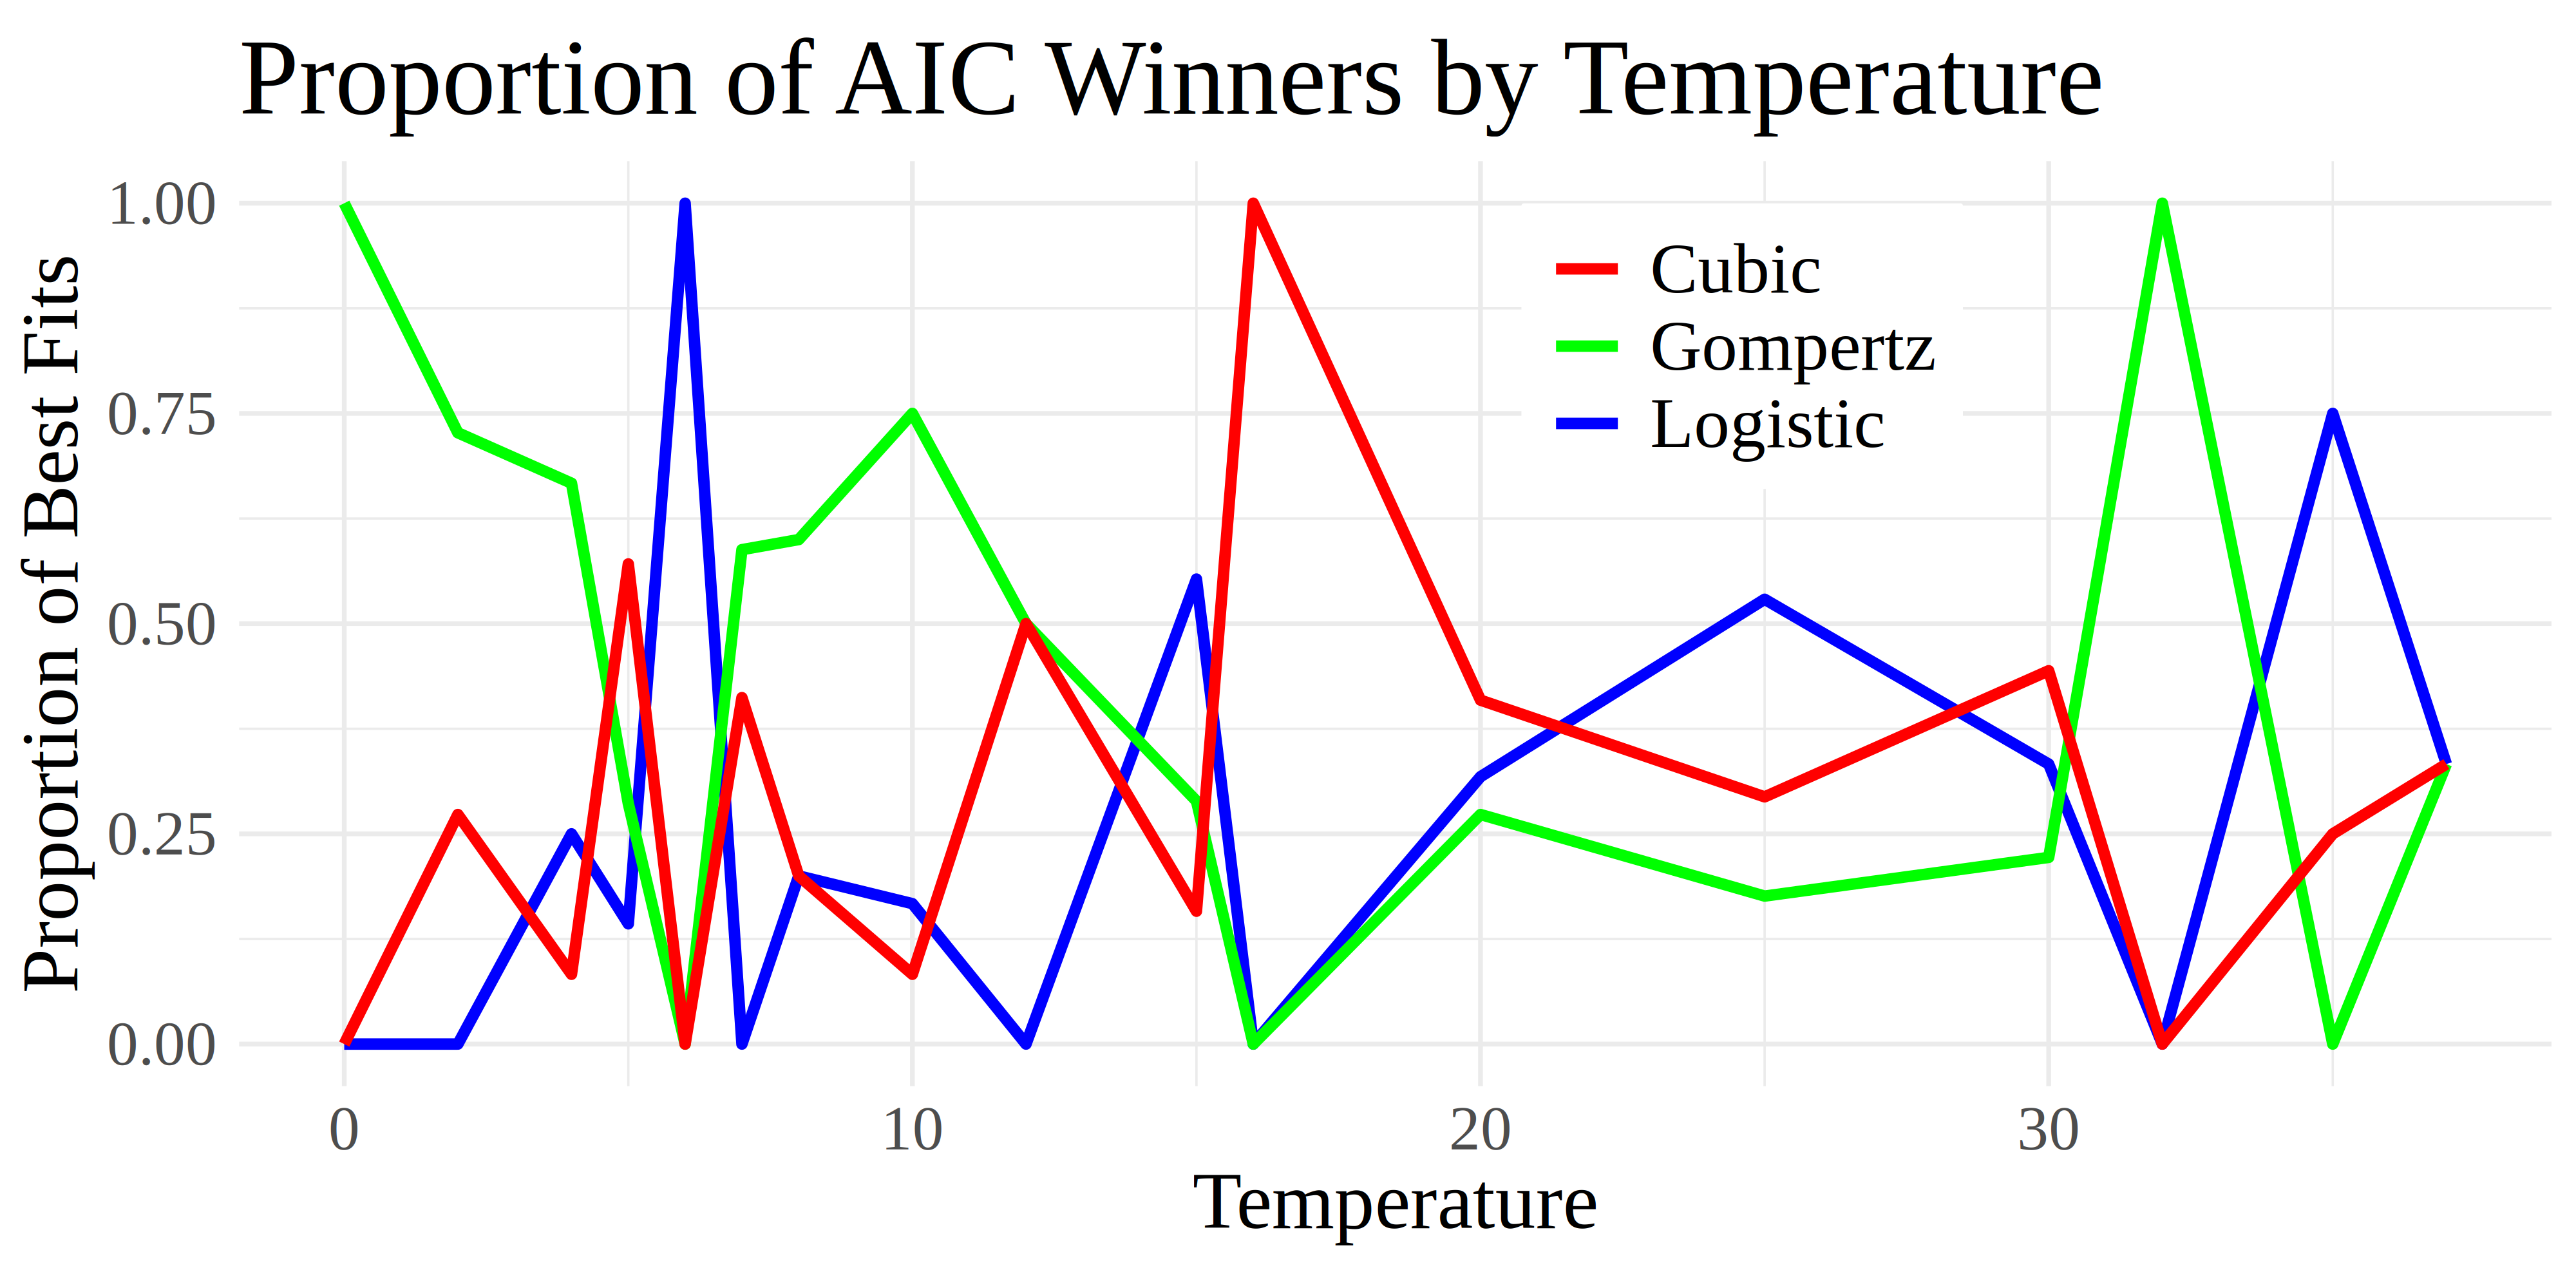
\includegraphics[scale=0.5]{proportionplot.png} 
  \caption{Line graph showing best model proportions against temperature}
\end{figure}
Observing the plot there is no clear trend between performance for any model and temperature. Whilst there are temperatures which certain models perform best at, for example cubic at 16 degrees, drawing definitive trends is challenging due to small sample sizes for each temperature.

\section{Discussion}

This study ultimately aimed to identify which models were best predictors of microbial growth at different temperatures to inform quantitative biologists, under which conditions should certain models be used for predictions. The Gompertz model was found to be the best predictor of microbial population growth - implying that the additional parameter compared to the Logistic model provides sufficient explanation of the data to justify extra model complexity. However, there was no evidence from figure 2 to suggest that the efficacy of any model is influenced by temperature. Therefore, this report encourages the use of the Gompertz model for predicting microbial populations across a range of temperatures.\\

The trade off between parsimony and complexity is an important dilemma to address in this case. Parsimonous theories advocate for simplicity of explanation \cite{Coelho2019} thus the most straightforward model that adequetly explains the data is best. Simplicity is often favoured as it is more interpretable and overfitting is less likely. In contrast, complex models with more parameters than its competitors (such as Gompertz) explain intricacies in the data, thus providing a better fit. Therefore, metrics that quantify the balance of parsimony and complexity, AICc and BIC, were used in this study to identify the best performing models. The inclusion of $\mathrm{R}^2$ in Table 1 highlights its insuitability and the need for parameter penalisation, as it expectedly more strongly favoured the cubic and Gompertz models than the other metrics.\\

The results do not align with the expectation that the Logistic model would outperform the Gompertz model at higher temperatures. Reasons for this may be due to the limitations of this study such as the other confounding factors at play. Firstly, the length and extent of different stages of microbial growth will depend on the environmental conditions relative to the conditions that it is best adapted for \cite{Dey2020}. For example, tlag increases for microbes placed in novel environments to allow for time taken to adapt to new conditions \cite{Rolfe2012}. This favours the Gompertz model where a tlag parameter is present. Secondly, growth mediums are known to affect metabolic rates in bacteria \cite{KIM201764}. Kim and Kim (2017) found that microbes grown in nutrient rich media had increased K and Rmax, and decreased tlags than those grown in nutrient poor media. This indicates that the Logistic equation is more suitable for nutrient rich media. To address the limitations of this study, more specified experiments that record enough data for each unique set of conditions would provide a more nuanced understanding of when each model works best.\\


The limited data set also reduces the significance of the findings of the study. Whilst the Gompertz model performed best for all criteria, no statistical analyses were conducted to address whether or not Gompertz would likely be the best performing model in another set of growth curves. Furthermore, the $\mathrm{A}_{\textit{W}}$ scores illustrate no overwhelming winner and therefore suggest model selection should be more specific to the conditions that a microbe is grown under. However, to combat the drawbacks of a limited dataset, the $\mathrm{A}_{\textit{W}}$ parameter estimations could be used to predict microbial population growth - particularly when there is no clearly best performing model. Model averaging using $\mathrm{A}_{\textit{W}}$ is mostly useful when multiple models exhibit roughly equal AICc values \cite{JOHNSON2004101}, so equally performing models are both considered when calculating parameters. This study generated Akaike estimated parameter values regardless of whether or not there was a clear best performer ($\mathrm{A}_{\textit{W}}$ $>$ 0.9). However, a potential improvement to the estimations, as suggested by Johnson and Omland (2004), would be to only use model averaging when the best performing models $\mathrm{A}_{\textit{W}}$ is less than 0.9. And otherwise just use the given parameters of the best performing model. This is to prevent the influence of poor performing models on parameter estimates.\\

Finally, whilst $\mathrm{A}_{\textit{W}}$ scores are great for model comparison and assessing relative performance. They do not illustrate how well each model really fits to the data as they are just probabilities. Therefore, their use alongside raw AICc or even $\mathrm{R}^2$ may be necessary. For example, through inspecting each growth curve used in this study (found in the plots directory), there are some instances where a death phase is present. Therefore, regardless of relative performance between Gompertz and Logistic models, both would have failed to capture a major phase of microbial population change.

\section{Conclusion}
In conclusion the results of this study provides explanation and evidence for why the Gompertz model should be used to gain a general idea of microbial population growth. Secondly, it is concluded that temperature does not influence model performance. However, it is likely that selecting models that perform best for particular conditions, or using $\mathrm{A}_{\textit{W}}$ is a more reliable method for predicting growth curves and parameters. The study also generated robust parameter estimates for Rmax and K (found in the supplimentary information) that may be used in future studies.

  \bibliographystyle{apalike}
  
  \bibliography{Bibliography}

  \end{document}









































































































































































































































































































































































































































































































































































































































































































































































































































































































































































































































































































































































































































































































































































































































































































































































































































































































